\documentclass[a4paper, 12pt]{article}
\usepackage{CJKutf8}
\usepackage{caption}
\usepackage[ruled,linesnumbered]{algorithm2e}
\usepackage{color}
\usepackage{indentfirst}
\usepackage{graphicx}
\usepackage{float}
\usepackage{amsmath}
\usepackage{amssymb}
\usepackage{amstext}
\usepackage{amsopn}
\usepackage{textcomp}
\usepackage{xcolor}
\usepackage{boxedminipage}
\usepackage{enumerate}
\usepackage{url}
\usepackage{times}
\usepackage{caption}
\usepackage{subfigure}
\usepackage{algpseudocode}
\usepackage{placeins}
\usepackage{comment}
\usepackage{multicol}
\usepackage{booktabs}
\usepackage{dblfloatfix}
\usepackage{bm}
\usepackage{hyperref}
\usepackage{titling} % 用於調整標題間距
\usepackage{titlesec}
\usepackage{array}   % for \renewcommand{\arraystretch}{1.5}
\usepackage{multirow}% for \multirow command
\usepackage{booktabs}% for better-looking tables
\linespread{1.5}
\setlength{\parindent}{2em}
\setlength{\hoffset}{0in}
\setlength{\voffset}{0in}
\setlength{\oddsidemargin}{0.05in}
\setlength{\evensidemargin}{0in}
\setlength{\topmargin}{0in}
\setlength{\headheight}{0.167in}
\setlength{\headsep}{0.333in}
\setlength{\textwidth}{6.268in}
\setlength{\textheight}{9.393in}
\setlength{\marginparsep}{0in}
\setlength{\marginparwidth}{0in}
\setlength{\marginparpush}{0in}
\setlength{\footskip}{0.5in}
\setlength{\droptitle}{-9em} % 調整標題與頁面頂部的距離

\input lstset.tex
\input macro.tex

\captionsetup[figure]{labelfont={bf},name={圖},labelsep=period}
% \captionsetup[table]{name={表格},labelsep=period}

\begin{document}



\begin{CJK}{UTF8}{bkai}
	\renewcommand{\abstractname}{\Large 摘要}
	\newcommand{\pluseq}{\mathrel{+}=}
	\title{以 LSTM 預測隨機亂數}
	\author{B093040007 張碩文}
	\date{}
	\maketitle
	\vspace{-4em}
	% Abstract
	\begin{abstract}
		在本專案中,會使用兩種生成隨機數的方式,分別為 LCG、linux /dev/random,生成好幾筆長度為 10000 的 0-9 之整數,讓 LSTM 以前面 5000 個 0-9 之亂數作為輸入,預測後 5000 個的 0-9 的整數,最後計算預測後的準確度,預期 LSTM 模型能學習到 LCG 生成隨機亂數的規則,而 linux /dev/random 的則無法學習其特徵,因為此隨機亂數本身是 truly random number,毫無規則性可言。
	\end{abstract}
	
	% Sections
	\section{研究動機}
	老師上課時提到 LCG 的演算法可用類似差分方程的方式表達,且上課時有 demo 過,在大部分的角度時,雖然 LCG 生成的亂數看起來雜亂無章,但是從側邊的某個角度看,卻發現有很明顯的三個平面,因此好奇擅長處理時序型資料的 LSTM 是否能透過 LCG 所產生的隨機亂數作為訓練資料,訓練後學習到 LCG 生成亂數的方式,若能準確預測,意味著亂數生成的方式過於簡單,可讓模型輕易的學習到其特徵,同時也用 linux 提供的 /dev/random,其本身為 truly random number 作為對照組,因為本身的生成方式是從環境中的物理上的雜訊蒐集而成,無任何規則性,預期模型無法從 /dev/random 學習到任何規則。 	
	\section{方法}
	\begin{figure}[tbh]
		\centering
		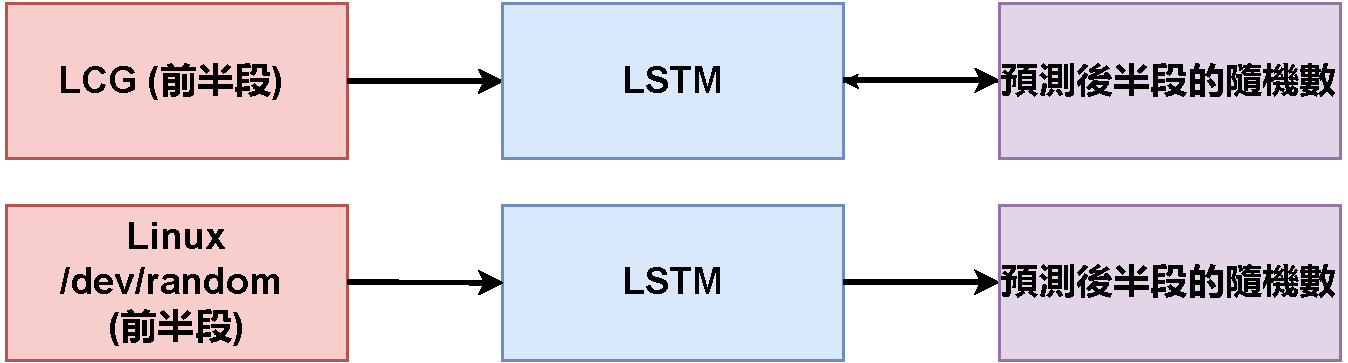
\includegraphics[width=0.7\textwidth]{src/NM_Architecture.pdf}
		\caption{架構圖}
		\label{fig-NM_Architecture}
	\end{figure}
	如\xfig{fig-NM_Architecture}所示,LSTM 模型的輸入為某隨機亂數序列的前半段,為 5000 個 0-9 之整數,模型預測為後半段 5000 個 0-9 之整數,且訓練 LCG 和 /dev/random 的模型架構完全相同,僅差在模型內部訓練後的權重會不同,且架構會使用 pytorch 本身提供的一些 pre-trained 模型,再使用 tranfer learning 使得模型的權重訓練成更適合此資料集。為了能清楚判斷是模型訓練結果不佳還是隨機亂數本身亂度夠高,會使用額外的亂數檢定法來分析亂數品質,像是 Monte Carlo value、Serial correlation coefficient、Entropy 等來衡量。
	\section{預期結果}
	預期模型能精準的預測 LCG 的隨機數,而 /dev/random 的則相反。
	\begin{table}[h]
		\centering
		\renewcommand{\arraystretch}{1} % adjust as needed
		\begin{tabular}{|c|c|c|}
			\hline
			分類 & 項目 & 金額 (NTD) \\
			\hline
			\multirow{3}{*}{戶外實境尋寶活動} & \multicolumn{1}{|c|}{尋寶遊戲設計與執行(含印刷費用)} & \$120,000 - \$160,000 \\
			\cline{2-3}
			& \multicolumn{1}{|c|}{工作人員薪資(時薪)} & \$50,000 \\
			\cline{2-3}
			& \multicolumn{1}{|c|}{影片宣傳和行銷} & \$100,000 \\
			\hline
			\multirow{3}{*}{改建\&活化建築} & \multicolumn{1}{|c|}{義村改造與設計} & \$500,000 \\
			\cline{2-3}
			& \multicolumn{1}{|c|}{藝術家設計\&裝置藝術} & \$250,000 \\
			\cline{2-3}
			& \multicolumn{1}{|c|}{岡山老街建築整修} & \$2,000,000 (optional) \\
			\hline
			\multirow{2}{*}{螺絲博物館費用} & \multicolumn{1}{|c|}{道覽服務} & \$20,000 \\
			\cline{2-3}
			& \multicolumn{1}{|c|}{DIY體驗材料費} & \$40,000 \\
			\hline
			\multirow{2}{*}{有獎徵答} & \multicolumn{1}{|c|}{宣傳和行銷} & \$25,000 \\
			\cline{2-3}
			& \multicolumn{1}{|c|}{購買獎項禮品} & \$50,000 \\
			\hline
			\multirow{2}{*}{其他} & \multicolumn{1}{|c|}{保險費用} & \$30,000 \\
			\cline{2-3}
			& \multicolumn{1}{|c|}{雜費} & \$30,000 \\
			\hline
			\multicolumn{2}{|c|}{總共費用} & \$3,000,000 \\
			\hline
		\end{tabular}
	\end{table}
	% \bibliographystyle{IEEEtran}
	% \bibliography{reference} 
	
\end{CJK}

\end{document}
